\chapter{Experiment I: Prospective Impressions}

\label{ch:option-results}

\Footnotetext{*}{Note: parts of this chapter have appeared in abridged form in \citep{Mawhorter2015b}.}

The goal of this chapter and the one that follows is to demonstrate \dunyazad/'s ability to manage player reactions by generating distinct choice structures.
%
Because of the way it uses answer set programming, \dunyazad/'s choice generation system not only generates choices, but itself constitutes a theory of choice poetics.
%
Survey data presented here thus not only validate that players' perceptions match \dunyazad/'s intent, but also inform the theory of choice poetics.
%
Statistical analysis of the data indicates that \dunyazad/ is largely successful in its goals, but also reveals some places where either the code, the theory, or both can be improved. 
%
These unexpected results are in fact one of the larger goals of \dunyazad/ as a project: by operationalizing choice poetics, \dunyazad/ enables experiments which can reveal details that wouldn't be obvious from simply observing human-authored choices, because as a computer program, \dunyazad/ makes \emph{inhuman} mistakes.


The results presented here are of course limited by \dunyazad/'s specificity: \dunyazad/ has a particular approach for creating e.g., \lbl{obvious} choices and information about properties of its \lbl{obvious} choices doesn't necessarily generalize to all obvious choices.
%
Largely, however, the extra considerations that this data suggests should be taken into account \emph{do} generalize, because they apply to any analysis or generation scheme which uses a particular subset of \dunyazad/'s constraints.
%
For example, one result that will be discussed suggests that when trying to figure out how players will evaluate different options, analysis in terms of absolute values is insufficient.
%
This result (which is unsurprising, as it echoes psychological research on real-life choices; see \citep{Schwartz2002}) clearly isn't something that's likely to be limited to just the particular choices that \dunyazad/ generates (in terms of genre or any other factor).
%
There might be some cases where humans do use only absolute value judgements, but until specific conditions under which this is true are found, it's safer to assume that both absolute and relative value judgements between options should be accounted for.
%
In any case, the discovery prompted by \dunyazad/ that absolute value judgements are insufficient for understanding choice poetics generalizes beyond the specifics of \dunyazad/'s choices.


The experiment presented here (and the experiment discussed in \cref{ch:outcome-results}) was set up in order to test \dunyazad/'s functionality and thereby also inform the theory of choice poetics that it is based on.
%
This first experiment is mainly concerned with prospective impressions, which are the result of the ``relative option analysis'' step in the goal-based choice analysis method described in \cref{sec:goal-based-choice-analysis}.
%
In \dunyazad/, these are represented using \prq{option\_feel}{} predicates, as described in \cref{sec:dunyazad-poetic-constraints}.
%
After analyzing the results of this experiment, I conducted a second experiment (discussed in \cref{ch:outcome-results}) focused on retrospective impressions, which are the results of retrospective analysis and are represented by \prq{outcome\_feel}{} predicates.
%
This chapter describes the details of the first experiment, including details of the experimental setup that are common to both experiments.


Both experiments broadly confirmed \dunyazad/'s abilities to generate the kinds of choices it was asked to, but also uncovered areas where it struggled.
%
In particular, \dunyazad/ has trouble balancing options to create true dilemmas because it does not have a sufficiently detailed model of player goal priorities, and it has trouble analyzing situations where multiple goals oppose each other, especially when such situations constitute a moral dilemma.
%
Additionally, it has trouble reasoning about actions which expend resources in service of a goal, and its indirect management of expectations can sometimes leave something to be desired.
%
All of these shortcomings suggest future work, of course, but also prompt reflection on the goal-based choice analysis method from \cref{sec:goal-based-choice-analysis}.
%
Accordingly, \cref{sec:results-prospective-caveats} revisits some of the concepts from goal-based-choice-analysis in light of the results from this experiment and the one presented in \cref{ch:outcome-results}.
%
The main takeaways for goal-based choice analysis are that humans should be careful to apply their faculties for comparing options in terms of things like moral imperatives and opportunity costs when analyzing options and outcomes.
%
Some other caveats are that relative option analysis is important in most situations, rather than only being needed when options are very similar, and that the outcome of an option can influence post-decision impressions of its desirability as an option pre-decision.

\section{Overview}

To exercise \dunyazad/'s prospective impressions system, I set up \dunyazad/ to construct three different kinds of choices:
%
\begin{itemize}
  \item \lbl{Relaxed} choices, where the stakes were low and there were no bad options.
  \item \lbl{Obvious} choices, where there was a single option that stood out as more advantageous than the rest.
  \item \lbl{Dilemmas}, where every option was about equally undesirable.
\end{itemize}
%
These three prospective impressions cover positive and negative option impressions, low- and high-stakes choices, and contrasting and similar option sets, so they exercise every dimension of player expectations that \dunyazad/ attempts to model.
%
Of course, the full set of \dunyazad/'s prospective impressions (shown in \cref{tab:prospective-impressions}) is broader, and there are plenty of prospective impressions that \dunyazad/ does not include definitions for, but \lbl{relaxed}, \lbl{obvious}, and \lbl{dilemma} choices were chosen as representative for this experiment.
%
Note that factors which give rise to ``obviousness'' or ``being a dilemma'' are quite a bit simpler than, say, factors that make a player feel regret.
%
These experiments, and indeed work on \dunyazad/ so far, has focused on these simple effects because if they can't be produced reliably, more complex effects are unlikely to work either.
%
The results presented here are thus only the first step in \dunyazad/'s use as a tool for exploring choice poetics.


After constructing choices, I ran a survey that asked participants to read a single choice generated by the system and answer some questions about their perception of the choice.
%
I analyzed the responses across choice categories and compared them against a uniform distribution to determine if players' perceptions match what the system intended.
%
The data show that \dunyazad/ was mostly able to produce the desired prospective impressions, but in a few specific cases there were surprising results.
%
Because \dunyazad/ is a transparent operationalization of the goal-based choice analysis technique described in \cref{sec:goal-based-choice-analysis}, both the expected and surprising results can usefully inform not only the system's development but also the theory of choice poetics.


\section{Method}

\label{sec:e1-method}

The primary goal of this experiment was to assess \dunyazad/'s ability to manage and predict player's prospective impressions, i.e., perceptions of a choice before making a decision.
%
To that end, the experiment focuses on players' perceptions of options at a choice, and does not even present outcomes to the participants at all.
%
The three choice types that were generated were chosen because they are each distinct in terms of the player expectations they engender, and because, as stated earlier, they together exercise \dunyazad/'s capacity to reason about stakes, positive and negative indicators, and both contrasting and similar options.


To gather data on player expectations, I generated choices using \dunyazad/, showed them to study participants, and asked participants a series of questions about specific qualities of the choice they just read.
%
Because I used Amazon Mechanical Turk to gather data, my participants were each paid a small amount and presumably approached the survey as a means to earn money rather than as a voluntary undertaking.
%
Because of this, questions were asked in a hypothetical manner (e.g., ``If you were reading this story, which option would you choose?'') rather than directly (e.g., by having participants pick an option) to imply that the task at hand was asking them to judge the choice as someone reading it for entertainment might.
%
Of course, this framing (and being asked specific questions in general) might encourage an analytical mode of engagement, which is not what \dunyazad/ is designed to support, but that limitation is to some degree inevitable when survey responses are solicited.


To control for participants paying little attention, being unfamiliar with English, or simply filling in random responses, two check questions were asked.
%
Responses from participants who failed to answer these questions satisfactorily were excluded from the analysis, as were responses where one or more questions were left blank (about 15\% of all participants).

\subsection{Treatments}

For this experiment, there were three experimental treatments, each corresponding to a different set of rules used by \dunyazad/ to generate the choice experienced by a subject.
%
These are the \obv{,} \rlx{,} and \dlm{,} choice types described above (see also \cref{tab:prospective-impressions} for formal definitions of these as \dunyazad/ perceives them).
%
The system definitions given in that section represent extra constraints placed on the choices generated by \dunyazad/ beyond its common core rules.
%
Each participant thus saw a choice shaped by one of three different constraint sets.


Of course, each constraint set can generate a potentially large range of specific choices, but this study was interested in perceptions common across choices generated using the same constraints.
%
One possibility would be to show each participant a unique choice from the space of choices possible given one of the treatment conditions.
%
However, this setup would mean that no single choice would be seen by more than one participant, and so there would be no way to analyze the contribution of individual choices to the perception of the different treatments.
%
Instead, I generated three different choices per treatment, and showed each choice to ten participants, for a total of 30 participants per treatment pre-attrition.

\begin{figure}[!h]
\quotebox{
  \quoteshape
You come to a tavern and decide to rest for a while. 
%
A merchant is bored and a noble is bored and an innkeeper seems knowledgeable. 
%
What do you do?
\begin{enumerate}[itemsep=0pt,topsep=4pt,parsep=0pt,partopsep=0pt]
\item You play a song for the noble \\
  (You have skill: musician. You have no tool for music).
\item You gossip with the innkeeper \\
  (You are missing skill: negotiation).
\item You play a song for the merchant \\
  (You have skill: musician. You have no tool for music).
\end{enumerate}
}
  \caption{An example choice.}
  \label{fig:results-exchoice}
\end{figure}

\subsection{Setup}

To set up the experiment, I used \dunyazad/ in its ``experiment'' mode (which causes it to generate only a single choice and to use a special framing) to generate three choices for each of the experimental conditions.
%
As an additional constraint, each choice was required to have exactly three options, so that the number of options wasn't a confounding factor in the data.
%
These nine choices were generated sequentially by the system, so there was no opportunity to cherry-pick ``good'' examples of each treatment category.
%
The choice shown in \cref{fig:results-exchoice} is the first choice that was generated; it is in the \dlm{} treatment.
%
The framing for each choice presented the skills that the system had assigned the player character for that choice, and established a basic context for the choice (see \cref{fig:exframing}).
%
The framing for each choice differed only in the skills presented and the fictional destination name, which \dunyazad/ chooses randomly from a fixed list of made-up names.


\begin{figure}[!h]
\quotebox{
  \quoteshape
You are about to set out on an epic journey. You are are heading towards towards the distant country of Jyv\"asky, hoping to earn fame and fortune.
%
You have some perfume and a book of legends, and you have skill: literacy, you have skill: musician, and you have skill: healing. 
%
Eager to be on your way, you set off on the road towards Jyv\"asky.
}
  \caption{Example framing. The repetition of ``towards'' is a typo that was present in the text shown to participants.}
  \label{fig:exframing}
\end{figure}


Once the choices were generated, their text was broken into parts and put into a comma-separated values file for upload to Amazon Mechanical Turk where the parts would be substituted into a template.
%
Given a survey template, Mechanical Turk generated individual survey pages for each question, and ten tasks were posted per question (a total of 90 tasks), which workers on Mechanical Turk were able to preview, accept, and fill out for payment (50 cents per task\footnote{
%
This was chosen based on online advice to pay about minimum wage for tasks on Mechanical Turk.
%
Given the median response time, the hourly pay rate was \$7.50, but in retrospect, the inconvenience of survey tasks (where a worker cannot complete the same task many times and thus work more efficiently) suggests that a higher pay rate would be appropriate.
%
For this reason (and because the second survey included more questions) I used a higher pay rate for the second experiment.
%
The total cost (about \$50 in this case, counting Amazon's 10\% fee) was quite cheap.}).
%
Myle Ott's ``uniqueturker'' script (\url{https://uniqueturker.myleott.com/}) was used to ensure that no individual worker filled out the survey more than once.
%
To avoid being targeted by bots, the tasks required workers with a 97\% acceptance rate across at least 1000 accepted tasks.

\subsection{Survey Content}

Each survey was divided into three sections.
%
The first section ``Preliminaries'' began with a prompt that read:
\begin{quote}
  \quoteshape
To provide useful data for this survey, you must be at least 18 years old and able to read English. To confirm this (and to confirm that you aren't a bot), please answer the following question.
\end{quote}
%
This section just contained the following question designed to ensure that subjects were at least 18 years old and had basic English proficiency:
%
\begin{quote}
  \quoteshape
If you're at least 18 years old, please don't write ``Age of years eighteen least at am I that confirm I,'' as the answer here, instead write that sentence backwards, ended with an exclamation point. If not, please do a different HIT, as I cannot use your data in my results, and thus I will not accept your response.
\end{quote}


The second section of the survey was titled ``The Choice'' and began with a prompt:
%
\begin{quote}
  \quoteshape
Please read the following short story which presents you with a choice, then answer the questions about that choice below.
\end{quote}
%
In this section, each survey displayed one of the nine generated choices, followed by a single multiple-choice question:
%
\begin{quote}
  \quoteshape
If you were reading this story, which option would you pick?
\end{quote}
%
This question had three options: ``Option 1,'' ``Option 2,'' and ``Option 3.''


The final section of the survey was titled ``Opinion Questions'' and began with a prompt:
%
\begin{quote}
  \quoteshape
Please rate your agreement with the following statements, from 1 (strongly disagree) to 5 (strongly agree).
\end{quote}
%
This section contained the following 8 Likert items in this fixed order\footnote{These were individual Likert items which did not compose a Likert scale, as the goal of the survey was to directly measure opinions, and there were no underlying psychological variables presumed to be giving rise to behavior.} (the quotes were part of the survey):
%
\begin{enumerate}
    \quoteshape
    \setstretch{1.2}
    \addtolength{\baselineskip}{0pt plus 1pt minus 1pt}
  \item ``There are no bad options at this choice.''
  \item ``There is a clear best option at this choice.''
  \item ``The stakes for this choice are low.''
  \item ``There are no good options at this choice.''
  \item ``All of the options at this choice are about equally promising.''
  \item ``There are options at this choice.'' (This is a trick question to test whether you're paying attention. Please simply indicate that you are in complete disagreement.)
  \item ``This is a difficult choice to make.''
  \item ``This choice feels like it will have important consequences.''
\end{enumerate}
%
Each question in this section was followed by the same five numbered options presented vertically:
%
\begin{enumerate}
    \quoteshape
    \setstretch{1.2}
    \addtolength{\baselineskip}{0pt plus 1pt minus 1pt}
  \item strongly disagree
  \item somewhat disagree
  \item neutral
  \item somewhat agree
  \item strongly agree
\end{enumerate}
%
For these questions (and the multiple-choice question in the previous section) participants selected an option by clicking a radio button next to that option. There were no default responses, so someone who didn't click any of the radio buttons would submit a blank response for that question.
%
Responses were treated as ordinal data, and labeled with the numbers 1 through 5 in the same order they appeared here (i.e. 1 $\rightarrow$ strongly disagree; 5 $\rightarrow$ strongly agree).

\section{Hypotheses}

\label{sec:e1-hypotheses}

Before conducting the survey, I came up with a set of initial hypotheses about how participants would answer these questions based on the treatment conditions.
%
There were three types of hypothesis: single-treatment hypotheses, between-treatment hypotheses, and stakes hypotheses.
%
Each singe-treatment hypothesis posited that under a particular treatment, respondents would generally agree with or disagree with a particular question.
%
The single-treatment hypotheses used are listed in \cref{tab:e1-single-treatment-hypotheses}.
%
Agreement with a question was determined by a one-sided Mann-Whitney-Wilcoxon U test \citep{Mann1947,Wilcoxon1945} against a uniform distribution%
\footnote{%
Another possible standard for comparison would be an all-neutral distribution.
%
Comparison against a uniform distribution helps demonstrate that the answers aren't random, however, and the unsupervised nature of the study meant that participants might have answered some questions at random in order to complete it quickly (although there were some other guards against this).
%
To verify that a uniform distribution was an acceptable standard I ran the same hypothesis checks against an all-neutral distribution and found that support for each was equal to or greater than support when comparing to the uniform distribution used.
}%
\ of responses with the alternate hypothesis being ``The median of the survey responses is significantly higher than the median of the uniform distribution.''
%
Disagreement likewise used a Mann-Whitney-Wilcoxon U test with the alternate hypothesis that the median of the survey responses was smaller than that of a uniform distribution.
%
In both cases, a confirmation of a hypothesis was taken to be significant for $p < 0.05$.


\begin{table}[!h]
\begin{center}
\bgroup
\def\arraystretch{1.3}
\begin{tabular}{p{19.9em} c c c}
\toprule
Question & Obvious & Relaxed & Dilemma \\
\midrule
\eIqIshort/    &     -    &  agree   & disagree \\
\eIqIIshort/   &  agree   &     -    & disagree \\
\eIqIIIshort/  &     -    &  agree   &     -    \\
\eIqIVshort/   & disagree & disagree &  agree   \\
\eIqVshort/    & disagree &     -    &  agree   \\
\eIqVIshort/   &     -    &     -    &     -    \\
\eIqVIIshort/  & disagree &     -    &  agree   \\
\eIqVIIIshort/ &     -    &     -    &  agree   \\
\bottomrule
\end{tabular}
\egroup
\end{center}
  \caption{Prospective single-treatment hypotheses by treatment}
  \label{tab:e1-single-treatment-hypotheses}
\end{table}


For the between-treatment hypotheses, survey data from two different treatments were compared using a Mann-Whitney-Wilcoxon U test to test whether one was statistically more-agreed-with than another (with the threshold for significance again being set at $p < 0.05$).
%
The statistics are the same for the converse cases, so only one test was performed per hypothesis (i.e., if responses to question 3 showed significantly more agreement for the \obv{} treatment than for the \rlx{} treatment, it follows automatically that they show significantly less agreement for the \rlx{} treatment than for the \obv{} treatment).
%
\Cref{tab:e1-between-treatment-hypotheses} lists the between-treatment hypotheses.
%
Across all 3 treatments, there were a total of 13 single-treatment and 9 between-treatment hypotheses.


%\begin{table}
%\bgroup
%\def\arraystretch{1.1}
%\begin{tabular}{l | c c c}
%Question & Obvious & Relaxed & Dilemma \\
%\hline
%\eIqIshort/    &      -     & $>$dil. &      -     \\
%\eIqIIshort/   & $>$dil. &      -     &      -     \\
%\eIqIIIshort/  &      -     &      -     &      -     \\
%\eIqIVshort/   &      -     &      -     & $>$both \\
%\eIqVshort/    &      -     &      -     & $>$obv. \\
%\eIqVIshort/   &      -     &      -     &      -     \\
%\eIqVIIshort/  &      -     &      -     & $>$both \\
%\eIqVIIIshort/ &      -     &      -     & $>$both \\
%\end{tabular}
%\egroup
%  \caption[Prospective between-treatment hypotheses by treatment]{Prospective between-treatment hypotheses by treatment The ``$>$'' signs indicate more agreement relative to the alternate treatment indicated by abbreviation. ``$>$both'' indicates that that treatment is hypothesized to be more-agreed-with than both other treatments individually (two separate hypotheses).}
%  \label{tab:between-treatments}
%\end{table}

\begin{table}
\bgroup
\def\arraystretch{1.3}
\begin{tabular}{p{19.9em} c}
\toprule
Question & Hypotheses \\
\midrule
\eIqIshort/    & relaxed $>$ dilemma \\
\eIqIIshort/   & obvious $>$ dilemma \\
\eIqIIIshort/  & - \\
\eIqIVshort/   & dilemma $>$ obvious \& relaxed \\
\eIqVshort/    & dilemma $>$ obvious \\
\eIqVIshort/   & - \\
\eIqVIIshort/  & dilemma $>$ obvious \& relaxed \\
\eIqVIIIshort/ & dilemma $>$ obvious \& relaxed \\
\bottomrule
\end{tabular}
\egroup
\caption[Prospective between-treatment hypotheses by treatment]{Prospective between-treatment hypotheses by treatment. The ``$>$'' signs indicate more agreement relative to an alternate treatment. ``$>$ obvious \& relaxed'' indicates that that treatment is hypothesized to be more-agreed-with than both of those treatments individually (two separate hypotheses).}
  \label{tab:e1-between-treatment-hypotheses}
\end{table}


The stakes hypotheses were simpler: across all treatments, participants who were shown a choice identified by the system as low-stakes should agree with the statement ``The stakes for this choice are low.''
%
Additionally, participants shown high-stakes choices were expected to disagree with that statement.
%
Both of these hypotheses were validated using Mann-Whitney-Wilcoxon U tests against uniform distributions as above.
%
A fall-back hypothesis for stakes was that participants who saw low-stakes choices would agree more strongly with that statement than participants who saw high-stakes choices (a between-cases hypothesis).


\section{Results}

\label{sec:e1-results}

Before processing the data from Amazon Mechanical Turk, responses that showed signs of inattentiveness, non-proficiency with English, or excess haste were filtered out.
%
In fact, as responses were being submitted, responses where either the age question was left blank or where the trick question (question 6) had an answer other than ``1 - strongly disagree'' or ``5 - strongly agree'' were rejected, meaning that Mechanical Turk would not pay the responder and the task would be reposted.
%
Including 6 rejected responses, a total of 96 responses were gathered, with 30 non-rejected responses to each treatment (10 per question).
%
Of the responses which remained, further filtering was performed:
%
\begin{itemize}
  \item Responses where the answer to question 6 wasn't ``1 - strongly disagree'' were dropped. These indicate a responder who isn't paying close attention to the survey.
  \item Responses where the total time spent on the task was less than or equal to 90 seconds were dropped. Answering all 8 questions in just 90 seconds is probably not possible if each question is given reasonable consideration. The median response time was 240 seconds (4:00) before filtering and 280 seconds (4:40) after filtering, although these times are simply the time between a participant accepting and submitting a task; they don't necessarily work on the task exclusively during that time, and in general accepting several tasks before doing them is a common pattern of behavior.
  \item Responses where any question was left blank were dropped. Given the ``neutral'' response option and the content of the survey, leaving a question blank is more likely a sign of lack of attention than of hesitation to answer.
\end{itemize}
%
After these filtering steps, a total of 79 valid responses remained, with 25 responses to the \obv{} treatment and 27 responses each to the \rlx{} and \dlm{} treatments.
%
Given these final response counts, I used a uniform distribution of 25 data points to test my single-treatment hypotheses, as that was the closest multiple of 5 (the number of response options) to the sizes of my data sets.
%
The low- and high-stakes conditions had 44 and 35 responses respectively; I used the same 25-point uniform distribution to test my stakes hypotheses.


\begin{figure}[!p]
  \centering
  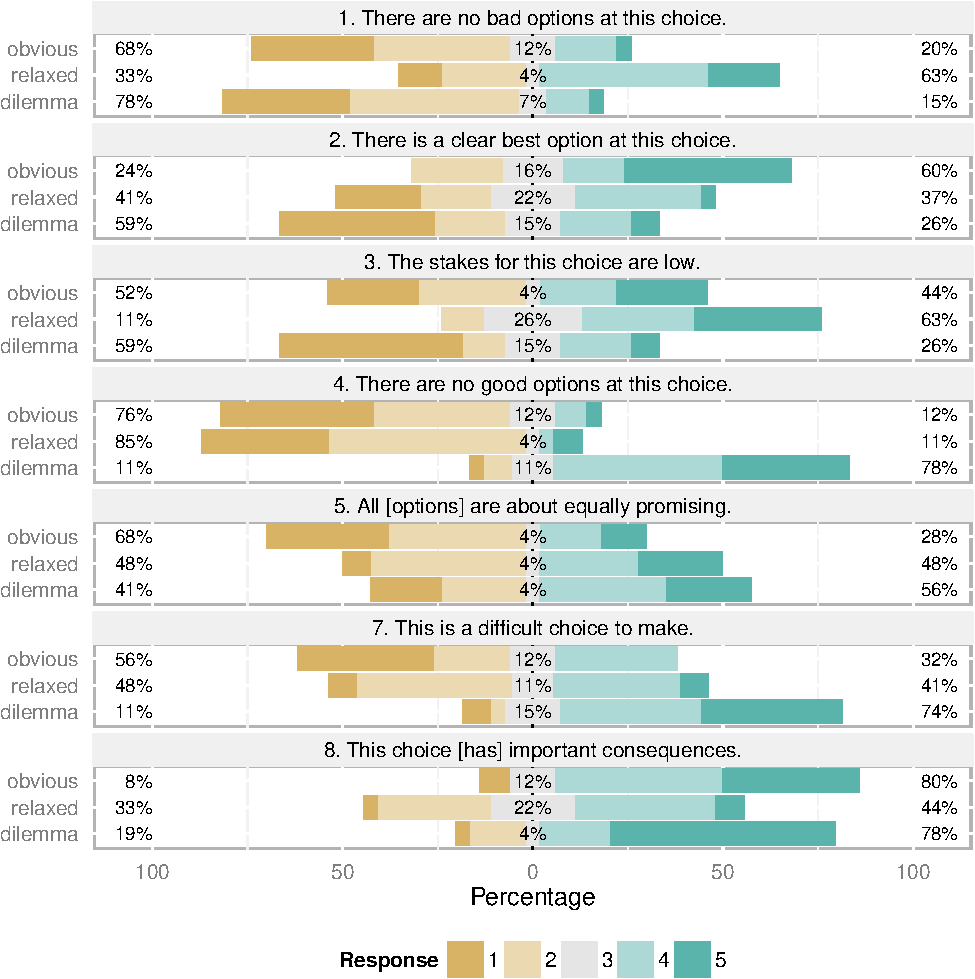
\includegraphics[width=\textwidth]{fig/combined-report-cropped.pdf}
  \caption[Prospective data summary]{A summary of the data by question plotted as percentages of respondents per treatment who gave each possible answer following \citep{Robbins2011}. Responses range from 1 (strongly disagree) to 5 (strongly agree) with 3 being ``neutral.'' Disagreeing responses are plotted to the left, and agreeing responses are plotted to the right.}
  \label{fig:e1-report}
\end{figure}

%\begin{table}[!p]
%  \centering
%\bgroup
%\def\arraystretch{1.3}
%%\setlength{\tabcolsep}{0.7em}
%%\begin{tabular}{l | p{0.5em} | p{2.2em} | p{1.8em} | p{0.5em} | p{2.2em} | p{1.8em} | p{0.5em} | p{2.2em} | p{1.8em}}
%\begin{tabular}{l | c|c|c | c|c|c | c|c|c}
%Question      & \multicolumn{3}{|c|}{Obvious} & \multicolumn{3}{|c|}{Relaxed} & \multicolumn{3}{|c}{Dilemma} \\
%\hline
%\eIqIabbr/    & \tenp & \tensig{A}{0.176} & \tesig{D}{0.009}{66\%} \\
%\hline
%\eIqIIabbr/   & \tesig{A}{0.023}{64\%}  & \tenp & \tesig{D}{0.047}{62\%} \\
%\hline
%\eIqIIIabbr/  & \tenp & \tesig{A}{0.015}{65\%}  & \tenp \\
%\hline           
%\eIqIVabbr/   & \tesig{D}{0.006}{68\%}  & \tesig{D}{0.005}{68\%}  & \tesig{A}{0.007}{67\%} \\
%\hline
%\eIqVabbr/    & \tensig{D}{0.069} & \tenp & \tensig{A}{0.322} \\
%\hline
%\hline
%\eIqVIIabbr/  & \tensig{D}{0.073} & \tenp & \tesig{A}{0.009}{66\%} \\
%\hline
%\eIqVIIIabbr/ & \tenp & \tenp & \tesig{A}{0.001}{71\%} \\
%\end{tabular}
%\egroup
%  \caption[Prospective experiment single-treatment results]{%
%Single-treatment results.
%%
%Each entry has a letter indicating the hypothesis (agree (A) or disagree (D)) followed by the $p$-value for that test.
%%
%Significant entries ($p < 0.05$) are listed in bold, and indicate a common-language effect size (the percentage of comparisons supporting the hypothesis).
%%
%Non-significant entries are highlighted in \nsighcolor/.
%%
%Note that question 6 (the trick question) is omitted here.
%}
%  \label{tab:e1-single-results}
%\end{table}

\begin{table}[!p]
\centering
{
\def\arraystretch{1.3}
\setlength{\tabcolsep}{0.4em}
\begin{tabular}{l  c  c c c  c  c c c  c  c c c}
\toprule
Question &%
 & \multicolumn{3}{c}{\eIobviousabbr/} &%
 & \multicolumn{3}{c}{\eIrelaxedabbr/} &%
 & \multicolumn{3}{c}{\eIdilemmaabbr/} \\
\midrule
\eInobadabbr/ &%
 & \tenp  &%
 & \tensig{A}{0.176} &%
 & \tesig{D}{0.009}{69\%} \\
\eIclearbestabbr/ &%
 & \tesig{A}{0.023}{66\%} &%
 & \tenp  &%
 & \tesig{D}{0.047}{63\%} \\
\eIlowstakesabbr/ &%
 & \tenp  &%
 & \tesig{A}{0.015}{67\%} &%
 & \tenp  \\
\eInogoodabbr/ &%
 & \tesig{D}{0.006}{70\%} &%
 & \tesig{D}{0.005}{70\%} &%
 & \tesig{A}{0.007}{69\%} \\
\eIbalancedabbr/ &%
 & \tensig{D}{0.069} &%
 & \tenp  &%
 & \tensig{A}{0.322} \\
\eIdifficultabbr/ &%
 & \tensig{D}{0.073} &%
 & \tenp  &%
 & \tesig{A}{0.009}{69\%} \\
\eIconsequencesabbr/ &%
 & \tenp  &%
 & \tenp  &%
 & \tesig{A}{0.001}{73\%} \\
\bottomrule
\end{tabular}

}
  \caption[Prospective experiment single-treatment results]{%
Single-treatment results.
%
Each entry has a letter indicating the hypothesis (`A' for agree or `D' for disagree) followed by the $p$-value for that test.
%
Significant entries ($p < 0.05$) are listed in bold, and indicate a common-language effect size (the percentage of comparisons supporting the hypothesis).
%
Non-significant entries are highlighted in \nsighcolor/.
%
Note that question 6 (the trick question) is omitted here.
}
  \label{tab:e1-single-results}
\end{table}


\begin{table}[!p]
\centering
\bgroup
\def\arraystretch{1.3}
\setlength{\tabcolsep}{0.7em}
\begin{tabular}{l c c c c}
\toprule
Question & Hypothesis & $p$-value & Effect \\
\toprule
\eInobadabbr/ &\tesig{relaxed$>$dilemma}{$\bm{3.1\sqtimes 10^{-4}}$}{76\%} \\
\midrule
\eIclearbestabbr/ &\tesig{obvious$>$dilemma}{$\bm{1.1\sqtimes 10^{-4}}$}{78\%} \\
\midrule
\multirow{2}{10em}{\eInogoodabbr/} &\tesig{dilemma$>$obvious}{$\bm{1.9\sqtimes 10^{-7}}$}{88\%} \\
 &\tesig{dilemma$>$relaxed}{$\bm{1.2\sqtimes 10^{-7}}$}{87\%} \\
\midrule
\eIbalancedabbr/ &\tesig{dilemma$>$obvious}{0.036}{64\%} \\
\midrule
\multirow{2}{10em}{\eIdifficultabbr/} &\tesig{dilemma$>$obvious}{$\bm{2.7\sqtimes 10^{-5}}$}{80\%} \\
 &\tesig{dilemma$>$relaxed}{0.001}{73\%} \\
\midrule
\multirow{2}{10em}{\eIconsequencesabbr/} &\tensig{dilemma$>$obvious}{0.140} \\
 &\tesig{dilemma$>$relaxed}{$\bm{3.8\sqtimes 10^{-4}}$}{75\%} \\
\bottomrule
\end{tabular}

\egroup
\caption[Prospective between-treatment results]{%
Between-treatments results.
%
Each row indicates a hypothesis, the corresponding $p$-value, and the effect size if the result is significant ($p < 0.05$). Significant results are shown in bold; non-significant results are in \nsighcolor/.
}
  \label{tab:e1-between-results}
\end{table}


A summary of the data is shown in \cref{fig:e1-report}.
%
The percentages shown are total percent of participants who disagreed, were neutral, or agreed with the given question (from left to right) and the percentages for each separate response are plotted as colored bars.
%
For each question, data from each of the three treatments is plotted separately, and in some cases divergence is immediately apparent.
%
Of course, differences that seem apparent on this summary graph may or may not be statistically significant.


I tested my hypotheses as described above, and the results of those tests are show in \cref{tab:e1-single-results,tab:e1-between-results}.
%
\Cref{tab:e1-single-results} shows the single-treatment hypothesis results: 9 of my 13 hypotheses were confirmed by my data, while 4 were not.
%
Each entry in this table indicates the hypothesis (agree $\rightarrow$ ``A'' and disagree $\rightarrow$ ``D''), the $p$-value for that hypothesis (the hypothesis is confirmed if the $p$-value is below 0.05), and if confirmed, the common-language effect size for that test.
%
\Cref{tab:e1-between-results} shows the between-treatment hypothesis results: 8 of my 9 hypotheses were confirmed by my data and 1 was not.


Note that the common-language effect size is just the percentage of comparisons between the cases being tested that support the alternate hypothesis.
%
This means that, for example, if all responses are neutral, the common-language effect size when asserting that the responses are greater than a uniform distribution will be exactly 50\% (the theoretical minimum common-language effect size).
%
This is because 50\% of comparisons between an all-neutral data set and a uniform data set will support the alternate hypothesis (that the neutral data's median is higher) and 50\% will refute it (counting tied comparisons as half-supporting and half-refuting).
%
By the same logic, if responses were all ``somewhat agree,'' the effect size would be 70\%, and if responses were all ``strongly agree,'' the effect size would be 90\% (the theoretical maximum effect size in the studies presented here).
%
The effect sizes listed in \cref{tab:e1-single-results} range from 62\% to 71\%, which are moderate to strong effects.
%
The effect sizes in \cref{tab:e1-between-results} range from 63\% to 83\%, with most being strong effects at $>$70\% effect size.


Besides the single-treatment and between-treatment hypotheses, all three of the stakes hypotheses were confirmed.
%
For the first (low-stakes choices would elicit agreement that their stakes were low) the $p$-value was 0.0047 and the effect size was 65\%.
%
The second stakes hypothesis (that high-stakes choices would elicit disagreement with the same statement) had a $p$-value of 0.0011 and an effect size of 70\%.
%
Finally, the backup hypothesis (that agreement would be higher in the low-stakes case than the high-stakes case) was a given as the first two were confirmed; it had $p = 9.7\times10^{-11}$ and an effect size of 83\%.


\section{Discussion}

Out of the 25 specific hypotheses, 20 were supported by the data.
%
This indicates that most of the perceptual qualities I expected given the constraints used to generate choices were in fact identified by most of the survey participants.
%
In particular, the fact that all of the stakes hypotheses were confirmed indicates that \dunyazad/'s author-based estimation of which player goals are more and less important is working.
%
On a treatment-by-treatment basis, the observed properties were:
%
\begin{itemize}
  \item \obv{} choices---Participants tended to agree that \obv{} choices had a clear best option (question 2) and they tended to disagree with the statement that they had no good options (question 4). I expected that participants would disagree that all of the options were equally promising (question 5) and that these choices were difficult (question 7) but in both cases the data did not confirm these expectations.
  \item \rlx{} choices---Participants tended to agree that the stakes for these choices were low (question 3) and they tended to disagree with the statement that these choices had no good options (question 4). I expected participants to agree that these choices had no bad options (question 1) but the data did not support this hypothesis.
  \item \dlm{} choices---Participants tended to disagree that there were ``no bad options'' at these choices (question 1) and agree that there were ``no good options'' at these choices (question 4). Furthermore, they disagreed with the statement that these choices had a clear best option (question 2), and agreed that these choices were difficult and had important consequences (questions 7 and 8). However, I expected participants to agree that all options at these choices were about equally promising, but the data did not support this hypothesis.
\end{itemize}
%
Overall, the data support \dunyazad/'s ability to control stakes and outcome valences, but also show that it has a bit of trouble making outcomes seem similar.
%
The areas where its choices were able to produce the desired poetic effects are important successes for automatic reasoning about choice poetics, and they imply that the goals survey participants considered when judging options align at least somewhat with those the system assumed players would have.


Places were the data did not support my hypotheses are opportunities for further scrutiny.
%
To start with, I wanted to investigate whether the failed hypotheses were the result of general trends across all choices generated under a treatment condition or whether any single choice contributed disproportionately to an unexpected result.
%
To do this I broke down the results by individual questions within a treatment and plotted them to see if there was any indication of per-question differences.


\subsection{Option Relativity}


\begin{figure}[!h]
  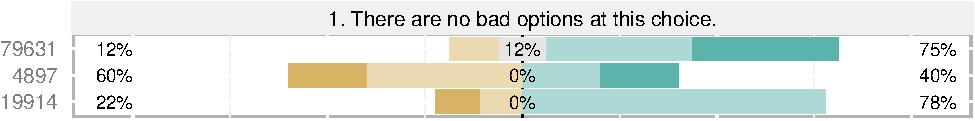
\includegraphics[width=\textwidth]{fig/relaxed-q1.pdf}
  \caption[``No bad options'' prospective responses]{A graph of responses to question 1 under the \rlx{} treatment. The three numbers are the seeds used to generate the three different choices for this treatment. The graph setup is the same as in \cref{fig:e1-report}.}
  \label{fig:e1-relaxedq1}
\end{figure}


The first of my failed hypotheses involved the \rlx{} treatment.
%
I expected the \rlx{} treatment to elicit agreement with the statement ``There are no bad options at this choice,'' but it didn't do so definitively (the statistical test failed to reject the null hypothesis that the answers to this question were consistent with a uniform distribution of underlying responses).
%
A per-choice breakdown of the data for the \rlx{} condition shown in \cref{fig:e1-relaxedq1} gives a strong indication that the question with seed 4897 elicited qualitatively different responses than the two other questions in this treatment.
%
That particular question is shown in \cref{fig:e1-seed-4897}, and reveals one possible reason for what I observed: unlike the other two questions in the \rlx{} case, option three of this question lists ``no relevant skills'' rather than giving a relevant skill possessed by the player.


\begin{figure}[!h]
\centering
\fbox{
\parbox{0.95\columnwidth}{
  \quoteshape
You come to a tavern and decide to rest for a while.
%
A noble is bored and a peasant is bored and a merchant is selling a book of herbal lore.
%
What do you do?
\begin{enumerate}[itemsep=0pt,topsep=4pt,parsep=0pt,partopsep=0pt]
\item You tell the peasant a story \\
  (You have skill: storytelling).
\item You tell the noble a story \\
  (You have skill: storytelling).
\item You offer to trade the merchant your dragon scale for the merchant's book of herbal lore \\
  (no relevant skills).
\end{enumerate}
}
}
\caption[``Relaxed'' choice 4897]{The \rlx{} choice with seed 4897 (minus the framing, which is largely the same as that shown in \cref{fig:exframing}).}
  \label{fig:e1-seed-4897}
\end{figure}


The fact that the player doesn't have any skills relevant to that action does not mean that the action will fail, but it might make that option seem less desirable than the others at that choice.
%
None of the options at the other two choices in the \rlx{} treatment listed ``no relevant skills,'' they all listed some skill that the player had as relevant, which explains why there might be a difference in responses.
%
If that wording caused the shift, it would be consistent with Schwartz et al.'s theory of satisficing versus maximizing personalities \citep{Schwartz2002} for real-world choices.
%
Schwartz et al. have found that while some people are happy as long as their choices lead to satisfactory results, others are unhappy if their choices lead to good but nevertheless suboptimal results.
%
The strong split in responses for this specific case (including both significant ``strongly disagree'' and significant ``strongly agree'' contingents) indicates that some people may be interpreting the phrase ``bad option'' as meaning options that are absolutely bad, while others may be comparing the options against each other.
%
It would take more data to discern whether this distinction is what is at work here, but it is clear that it is an important distinction for choice poetics, and it is not yet something that \dunyazad/ reasons about.


Although \dunyazad/ does not reason about this, it is to some degree aware of the distinction between the question with seed 4897 and the other two questions in that treatment.
%
The constraints for the \rlx{} condition were that each option either ``enables'' or ``achieves'' a goal (in the technical senses; see page \pageref{page:option-analysis} in \cref{page:option-analysis}), and in this case, the system generated two options that ``achieved'' a goal and one that merely ``enabled'' a goal, thus creating a distinction even on its own terms.
%
The other two questions in the \rlx{} category each included three options which ``achieved'' a goal.
%
In light of the survey results, it is clear that to construct choices that unambiguously have ``no bad options'' the system should not only require that each option works towards a player goal, but that each option is balanced against all others.

\subsection{Balancing Failures}

Another unsupported hypothesis was that in the \dlm{} treatment participants would agree with the statement ``All of the options at this choice are about equally promising.''
%
I expected this because one of the constraints of the \dlm{} treatment was that all of the threatened goals should have the same priority.
%
However, even for the individual choice in the \dlm{} treatment where participants reported the most agreement, 30\% of participants answered ``somewhat disagree.'' 


\begin{figure}[!h]
  \centering
  \includegraphics[width=0.8\textwidth,page=3]{fig/choices-cropped.pdf}
  \caption[Histogram of option preferences for ``dilemma'' choices]{A histogram of options selected by participants at the three different \dlm{} choices (each labeled by seed).}
  \label{fig:e1-dilchoices}
\end{figure}


\Cref{fig:e1-dilchoices} shows the options that participants said they would choose for the three dilemma choices.
%
For the first two choices, option two is a clear loser, and looking at the choices, it's easy to see why.
%
Both of those choices (which are nearly identical) involve being attacked by a dragon.
%
In both choices, option two is an option to attack the dragon yourself, but of course you have neither the ``fighting'' skill nor a weapon, and the dragon has both.
%
Although you also lack relevant skills for the other options, making a desperate attempt to flee from or pacify a dragon seems like a better choice than fighting it (at the very least, it did to all of my participants).


There are three factors contributing to the system's divergence from players' analysis of the options.
%
The first has to do with the granularity of expectations, the second with the granularity of goal priorities, and the third with stacking goals.


First, there are some clear arguments available to players as to why fighting might be a worse option than fleeing (for example) in an unfavorable situation.
%
One is that fighting presents a \emph{greater risk} of a bad result, and another is that fighting is directly related to a \emph{categorically worse} result.
%
The first argument has to do with the granularity of expectations: \dunyazad/ just recognizes events as \prq{unlikely}{,} \prq{neutral}{,} or \prq{likely}{.}
%
In this case, it reasons that since both fleeing and fighting are \prq{likely}{} to \prq{fail}{} the goal of avoiding the present threat, both options fail a high-priority goal.
%
However, given that all options are marked negatively, the prospect of fleeing evokes more hope for unwarranted success than the prospect of fighting.
%
This could be expressed in \dunyazad/ by introducing evaluations like \prq{somewhat\_likely}{} and \prq{very\_likely}{} that would distinguish these cases.
%
The \prq{skill\_link}{} mechanism would have to be updated to give estimates of these levels of likelihood for different actions in different circumstances, of course.


Another argument a player could make as to why fighting is worse than fleeing in this situation has to do with the relative magnitude of the results.
%
Internally, \dunyazad/ recognizes that the \prq{attack}{} option is likely to \prq{fail}{} both the \prq{avoid\_threats\_to}{} and \prq{preserve\_health}{} goals, while the \prq{flee}{} option is only expected to \prq{fail}{} the \prq{avoid\_threats\_to}{} goal.
%
However, as \dunyazad/ is written now, it treats an option that indicates one high-priority goal failure no differently form one that indicates multiple failures.
%
Particularly for choice structures which are supposed to have balanced options, some kind of counting logic would be useful to determine when one option is better or worse than another, even when they're in the same general category.


In the same vein, one could argue that even without counting how many goals fail, the \prq{preserve\_health}{} goal should be higher-priority than the \prq{avoid\_threats\_to}{} goal.
%
In part because of complexity concerns (although I have not tested this extensively) I made a decision to limit \dunyazad/ to two priority levels.
%
One could imagine instead a partially directed ``more-important-than'' graph between all player goals at each timepoint, which would be another way for \dunyazad/ to realize that fighting is worse than fleeing in this case.


The problem here is that the system's representation of player expectations is not fine-grained enough.
%
To the system, all of the options at these choices are expected to ``fail'' the player's goal of keeping their character alive and uninjured, but the system makes no distinction beyond that.
%
How certain does such failure seem to the player?
%
Exactly how badly does the player expect to fare when their goal is not met?
%
In this case, even when told that the situation is hopeless (or perhaps especially then), fleeing seemed a better option than attacking the dragon head-on, but the system doesn't distinguish those cases.
%
Based on this data, the system should be improved by adding more detail to its assessments of goal failure and success.


Any one of these corrections would help this particular case, but especially given that \dunyazad/ also has difficulty producing balanced positive options as mentioned in the previous sub-section, I suspect a more focused approach would be better.
%
After all, the likelihood reasoning \emph{is} doing a good job of predicting which options players will view positively or negatively; it just has a hard time figuring out whether options are equally positive or equally negative.
%
Rather than further overload the current reasoning, an additional subsystem dedicated to direct relative analysis of options should be added.
%
This system could separately maintain more-nuanced representations of goal priorities and outcome likelihoods, and then build arguments as to why each option is more- or less-desirable than each other option.
%
In many cases, this nuanced relative analysis could be short-circuited when the old low-fidelity analysis detects a difference.


In terms of the choice analysis method presented in \cref{ch:choice-poetics}, this exact problem was already mentioned in \cref{sec:cp-relative-option-analysis} (see the second paragraph where it talks about the balance of impacts).
%
I hypothesized here that \dunyazad/ would be able to fake a more detailed analysis by just insuring that the threatened goals had equal stakes, but that turned out not to be true.
%
In this case, what was learned from \dunyazad/'s failure backs up the theory: dilemmas are a case which needs closer inspection.
%
Getting this experimental result is still useful, because it provides a concrete example of why this is the case.


\subsection{Outcome Clarity}


\begin{figure}[!p]
  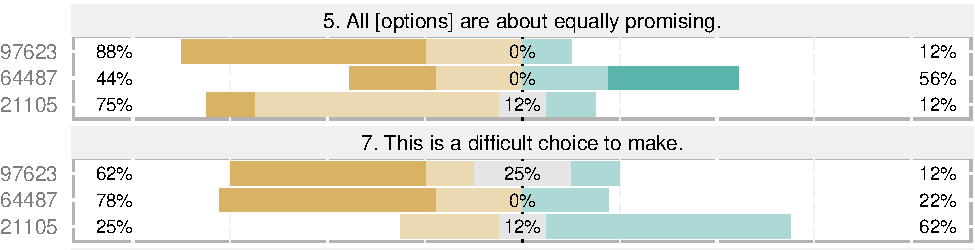
\includegraphics[width=\textwidth]{fig/obvious-q5-q7.pdf}
  \caption[Prospective balance and difficulty responses for ``obvious'' choices]{A graph of responses to questions 5 and 7 under the \obv{} treatment by seed. For question 5, the choice with seed 64487 is clearly different from the other two, and for question 7, the choice with seed 21105 is the one that stands out. \Cref{fig:e1-seed-64487,fig:e1-seed-21105} show the text of the divergent choices.}
  \label{fig:e1-obviousq57}
\end{figure}

\begin{figure}[!p]
\centering
\fbox{
\parbox{0.95\columnwidth}{
  \quoteshape
You come to a tavern and decide to rest for a while.
%
A merchant is bored and a peasant seems knowledgeable and an innkeeper seems knowledgeable.
%
What do you do?
\begin{enumerate}[itemsep=0pt,topsep=4pt,parsep=0pt,partopsep=0pt]
\item You gossip with the innkeeper \\
  (You are missing skill: negotiation).
\item You tell the merchant a story \\
  (You have skill: storytelling).
\item You gossip with the peasant \\
  (You are missing skill: negotiation)
\end{enumerate}
}
}
\caption[``Obvious'' choice 64487]{The \obv{} choice with seed 64487.}
  \label{fig:e1-seed-64487}
\end{figure}

\begin{figure}[!p]
\centering
\fbox{
\parbox{0.95\columnwidth}{
  \quoteshape
You come across some bandits attacking a merchant.
%
The bandits are threatening the merchant.
%
What do you do?
\begin{enumerate}[itemsep=0pt,topsep=4pt,parsep=0pt,partopsep=0pt]
\item You attack the bandits \\
  (They have skill: fighting. You are missing skill: fighting. They have no tool for fighting).
\item You travel onwards \\
  (no relevant skills).
\item You talk the bandits down \\
  (no relevant skills).
\end{enumerate}
}
}
\caption[``Obvious'' choice 21105]{The \obv{} choice with seed 21105.}
  \label{fig:e1-seed-21105}
\end{figure}


Not only did I expect participants to agree that options were balanced for \dlm{} choices, but I also expected them to disagree for \obv{} choices.
%
Here again my hypothesis was not supported by the data.
%
A per-choice analysis of question 5 in the \obv{} condition (the top half of \cref{fig:e1-obviousq57}) shows that again, one choice is divergent from the other two.
%
\Cref{fig:e1-seed-64487} shows that middle choice, which compared to the other two \obv{} choices is low-stakes (one of the other choices starts with a dragon attack, the other with bandits attacking some merchants).



Not only are the stakes for this choice low, but they are unclear.
%
What exactly does the player hope to gain by gossiping or by telling a story?
%
Perhaps friendship or some useful information, but those potential rewards seem both uncertain (even given a ``successful'' action) and questionably useful.
%
In contrast (albeit a contrast that participants did not see directly) the utility of fleeing from an attacking monster is clear, even if it is uncertain whether you will succeed.
%
Furthermore, there aren't any obvious risks associated with options 1 and 3, so even if the player is missing a relevant skill, they might still be worth trying.
%
Given this combination of low stakes, a dubious reward for the most-successful-seeming option, and seemingly consequence-free options all around, it is not hard to see how some might find these options ``about equally promising.''


On the other hand, the system's attempt to construct an obvious choice in this case was still somewhat successful.
%
7 of 9 participants who saw this choice ``strongly agreed'' with the statement ``There is a clear best option at this choice'' and 8 of those 9 picked option \#2 as the option they would choose.
%
While it might seem like a contradiction to agree (as 3 participants did) with both the statement that a choice has equally promising options and the statement that it has a clear best option, this highlights the difference between outcomes-focused evaluation of individual options and choice-oriented option comparison.
%
The phrasing of ``All of the options at this choice are about equally promising,'' suggests evaluating each option independently and comparing those values roughly.
%
In contrast, ``There is a clear best option at this choice,'' suggests comparing the options against each other to find one that is better than the others.
%
The fact that people often make decisions inconsistent with simple utility calculation is well-known (see e.g., \citep{Tversky1993}), so it should not be surprising that a context in which someone is asked to make a decision might elicit a different response than a context in which someone is asked to rate responses.


The implications for choice poetics are interesting, because choice poetics is concerned with both mindsets.
%
At least in terms of impact on the player, there's clearly a difference between a choice where all of the options seem ``about equally promising'' and where that's definitely not the case, even if both choices have ``a clear best option.''
%
Choices where options seem equally promising but most players choose a particular route regardless might even be good candidates for the focus of regret.
%
For example, if it turns out that the ``clear best option'' leads to failure and players are forced to revisit the original decision, having seen some potential in the alternatives they're more likely to feel that the choice was fair, and thus presumably blame their own decision for the consequences (\cref{sec:results-about-regret} discusses some data relevant to this point that resulted from the experiment on outcome evaluations).
%
At the same time, if the designer can be confident that most players will go down the ``obvious'' route first even without making the contrast with the other options huge, they can assume that most players will experience the regretful path as opposed to choosing the ultimately correct option the first time.


Despite the interesting revelations prompted by this case, \dunyazad/ does actually have a problem here: it is analyzing outcomes according to the game mechanics that it knows about, but the players in this case aren't playing a game: they're experiencing a single choice with very little context.
%
If someone had played a few of \dunyazad/'s output stories already, they'd have a view of the possibility space much more similar to \dunyazad/'s, especially in terms of the outcomes of actions like \prq{gossip}{} and \prq{tell\_story}{.}
%
If the players knew what to expect from both success and failure at these actions, and had a stronger sense of the role skills play in determining outcomes, they wouldn't get their hopes up, and the choice \emph{would} be ``obvious.''


That is the deeper issue here as well: the simple notions of ``success'' and ``failure'' when performing an action often don't correspond to overall positive an negative results when an action isn't clearly oriented towards some pressing player goal.
%
For example, an attempt to ``gossip'' despite lacking the relevant skill seems like it might still yield interesting results, and it isn't likely to be disastrous.
%
The same is not true of attacking an enemy: when they're more skilled or better-armed, there's a clear sense of danger (and of what is at stake).
%
In other words, \dunyazad/ is doing a good job of manipulating player expectations when it is heavy-handed, threatening high-priority player goals to make options appear hopeful or doomed.
%
However, when \dunyazad/ attempts to use low-priority goals in the same fashion, players don't follow its lead: ``My gossiping probably won't go `as intended?' Well, it might still be awesome!''


The simplest response to this is to just tread carefully when creating using low-stakes choices and assume that some of them aren't going to get the result you want, while making sure to use high-stakes choices if a particular property like obviousness is critical.
%
In the longer term, \dunyazad/ should recognize things like the desire to explore rather than always travel the beaten path (especially when the stakes are low).
%
At the same time, one area for future work is goal-probing questions, which would allow \dunyazad/ to ask the player (either directly or indirectly) to indicate their goals.
%
These questions would serve two purposes: first, they would allow \dunyazad/ to dynamically determine which goals (including low-priority goals) the player thinks are important.
%
Second, these questions, when successful, may subtly influence players by committing them to a goal: one a player affirms a goal, they may be more likely to behave in a manner consistent with that goal in the future (see e.g., \citep{Hall2012} on the powerful instinct for post-hoc justification when an opinion is perceived---even incorrectly---to be one's own).


\subsection{Conflicting Goals}


My hypothesis that respondents would not find \obv{} choices difficult highlights a different choice in the \obv{} category.
%
The data did not support this hypothesis, and as shown in \cref{fig:e1-obviousq57}, the choice with seed 21105 accounts for the majority of all responses that contradict it.
%
That choice is shown in \cref{fig:e1-seed-21105}, and from the system's perspective, it satisfies the definition of an obvious choice (see \cref{tab:prospective-impressions}) because the second option ``achieves'' a player goal, while neither the first nor the third do, and both the first and third ``threaten'' a player goal.


The perceived difficulty of this decision probably stems from the fact that it pits two player goals against one another: the goal of self-preservation is best served by option two, but the goal of helping others in need is best served by one of the other options.
%
This is similar to the lack of distinction between threatening one and two goals encountered above.
%
Even when one option at a choice clearly has the most-positive outcome for the player considering all goals to be equal, when that choice pits multiple goals against one another, it may be very difficult indeed.
%
In fact, choices with these structures may give rise to an entirely different set of poetic concerns that involves moral judgements (this is exactly how morality thought experiments like the ``trolley problem'' are constructed, for example---see \citep{Thomson1976}).
%
A difficult decision between two desirable or undesirable outcomes feels completely different from a decision between two outcomes each justified by competing moral principles, and it can resonate powerfully to the broader narrative structures of a story.
%
In its current state, \dunyazad/ doesn't reason about morality at all: it makes no distinction between goals in terms of their root motivations, and it has no compunction about how a result is achieved as long as no player goals are threatened in the process.
%
While \dunyazad/ gets perhaps surprisingly far without these capabilities, they're clearly important and can come up by accident even when \dunyazad/ isn't trying to make use of them.


That said, a detailed inspection of the answer set that resulted in this choice reveals another problem with the system: ignoring the lack of moral reasoning, it's simply not working as intended.
%
In this case, \dunyazad/ actually thinks that travelling onwards serves the goal of preventing the threat to the merchant (because if the player travels onwards, that entire situation is left behind and therefore the threat no longer exists) while it has no conception that this serves a goal of self-preservation (although it understands that interfering by either means threatens the player's safety).
%
There are thus two more changes to the system suggested by this data: first a bug-fix related to the consequences of travelling onwards, and second, the addition of relative goal relevance across options: the idea that if all but one option threatens an important goal, then the remaining option can be seen as indirectly supporting that goal even if none of its outcomes directly further that goal.
%
Without running this experiment, I would eventually have found and fixed the ``travel onwards'' bug, but I may not have thought to make the second change.
%
In this case, the data served to help find and diagnose an anomaly in my system, which turned out to involve an error in the code, but at the same time also pointed to two future goals for the choice structure model: adding explicit moral reasoning, and a notion of relative goal relevance when all but one option relates to a goal in the same way.


\subsection{Stakes and Consequences}

The final unsupported hypothesis was that participants would feel more strongly that \dlm{} choices had important consequences than that \obv{} choices did.
%
This hypothesis was based on the idea that consequences might seem more relevant (and thus important) when a decision was more difficult.
%
Given that one of my \obv{} choices seemed difficult to many participants as discussed above, it is unsurprising that this hypothesis was not supported.


\begin{figure}[!h]
  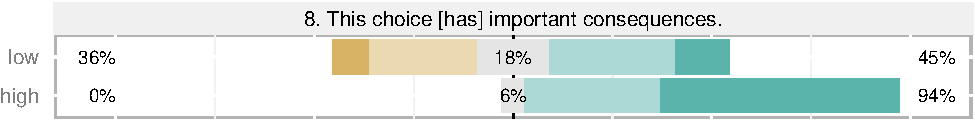
\includegraphics[width=\textwidth]{fig/stakes-q8.pdf}
  \caption[Prospective consequences results by stakes]{A graph of responses to question 8 across all treatments by stakes.}
  \label{fig:e1-stakesq8}
\end{figure}


What is interesting is the effect of the choice stakes on this question.
%
The similar hypothesis that participants would agree more in the \dlm{} case than the \rlx{} case \emph{was} supported by the data, and one big difference between those two treatments is the stakes associated with them.\footnote{A statistical analysis of the assertion that participants agree more with the statement that a choice's stakes are low in the \rlx{} case than the \dlm{} case (not one of my original hypotheses) reveals a strong significant effect ($p = 2.88\times10^{-5}$; effect size 76\%).}
%
In fact, when analyzing the data for question 8 according to stakes rather than the three treatments, high-stakes choices overwhelmingly seem as if they will have important consequences, while low-stakes choices are mixed (see \cref{fig:e1-stakesq8}).


Statistics confirm the obvious: not only did the high-stakes condition elicit significantly more agreement on question 8 than the low-stakes condition ($p = 2.14\times10^{-8}$; effect size 79\%), it was also significantly above a uniform distribution ($p = 4.9\times10^{-6}$; effect size 78\%).
%
Because all of the \rlx{} choices were low-stakes by design, there is of course correlation between the stakes and the treatments, but the 35 high-stakes cases were about evenly distributed between the \obv{} and \dlm{} treatments (16 in \obv{} and 19 in \dlm{}).
%
Such an overwhelming effect (none of the 35 respondents who saw a high-stakes choices thought it would \emph{not} have important consequences) further indicates that the system is successful in predicting high-stakes player goals: for 94\% of choices where the system thought that an important player goal was affected, players agreed at least somewhat that the consequences seemed important.


\section{Conclusions}

Overall, this study confirmed \dunyazad/'s ability to construct choices based on player expectations when certain criteria are met.
%
Notably, many of the failed hypotheses involved situations where several options together affected how a choice was perceived:
%
\begin{itemize}
  \item For question 1 (``There are no bad options at this choice.'') relative rather than absolute judgements of what is a ``bad'' option may have come into play.
  \item For question 5 (``All of the options at this choice are about equally promising.'') it seems \dunyazad/ may need to make finer distinctions between different modes of goal failure, as several options expected to lead to failure may still seem to offer a range of possibilities when no better options are present.
  \item Question 7 (``This is a difficult choice to make.'') showed that a choice can be difficult when multiple goals conflict, even when expectations for one goal are much better than for another.
\end{itemize}
%
These results point to several possible improvements for \dunyazad/, and collectively reinforce the importance of considering choices holistically when evaluating choice poetics.


As already discussed, there are a number of changes that could be made to \dunyazad/ based on these results:
%
\begin{itemize}
  \item Implement separate ``satisfaction'' and ``maximization'' player decision modes so that the system can reason about how difficult a decision might seem, whichever decision modality a player is using.
  \item Upgrade \dunyazad/'s system for estimating how individual options affect goals by adding more detail so that it can further distinguish different magnitudes of risk and reward.
  \item Have \dunyazad/ represent players' uncertainty about the possible outcomes of actions like ``gossip'' and ``tell story'' so that it can have a clearer picture of which options seem promising in low-stakes situations.
  \item Implement goal-probing questions (either direct or indirect) that allow the system to gain direct knowledge about player goals, especially for low-stakes options. This would also allow \dunyazad/ to further support role-playing by allowing different players to choose options which imply different goals or goal priorities.
  \item Implement a model of goal conflicts and more detailed relative goal priorities including moral reasoning.
  \item Implement the idea of relative goal relevance: if all but one option at a choice either threatens or enables a goal, then the remaining option implicitly does the opposite.
\end{itemize}
%
These changes could make \dunyazad/ even more successful at constructing choices which produce particular player expectations (and thus which can produce specific poetic effects).
%
They are also in line with my goal of getting \dunyazad/ to generate choices with more complex poetics, such as choices that elicit regret or prompt deliberation.


One important functionality of \dunyazad/ not tested in this first study was its ability to judge outcomes.
%
This study did largely verify that \dunyazad/'s player expectations about options are working, and it can generate outcomes that both support and betray those expectations.
%
The experiment described in \cref{ch:outcome-results} relies on this functionality to test how accurate \dunyazad/'s estimates of retrospective perceptions are.
